%location/filename: tex/fig/ap1.tex
%author: Anders Østevik
%Last edited: 20.05.2016
%#######--Appendix - HSMC-to-VLDB gerber files--#######
%

\documentclass[main.tex]{subfiles}

\begin{document}

\chapter{Schematic and PCB Layout} 

The schematic of the HSMC-to-VLDB PCB is shown in figures \ref{fig:pcb_sch1}, \ref{fig:pcb_sch2} and \ref{fig:pcb_sch3}. The PCB layout is shown in figures \ref{fig:pcb_tb} and \ref{fig:pcb_in}.

\begin{sidewaysfigure}[H] % H(strictly put HERE > h!)
\begin{center}
% h(here), !(force), t(top), b(bottom), p(on extra page)
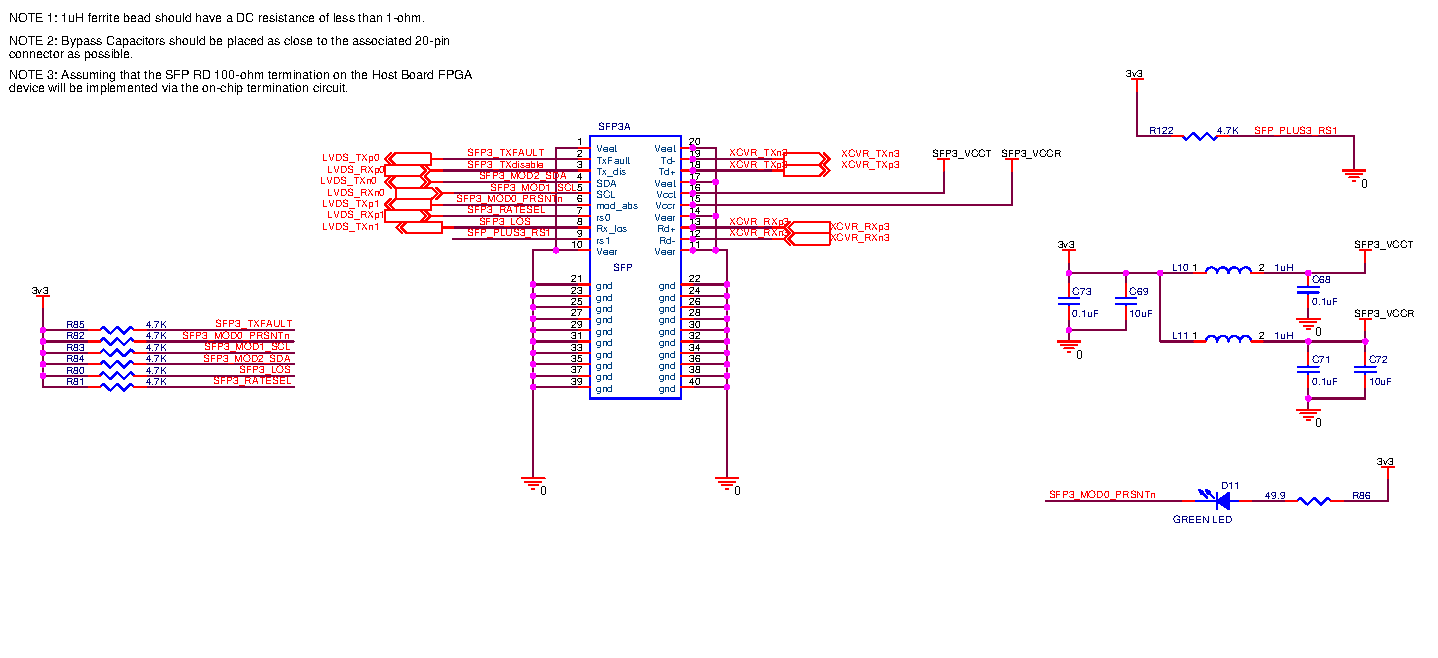
\includegraphics[width=1\linewidth]{../img/pcb_sch1}
\caption{PCB Schematic, SFP connector.}
\label{fig:pcb_sch1}
\end{center}
\end{sidewaysfigure}

\begin{sidewaysfigure}[H] % H(strictly put HERE > h!)
\begin{center}
% h(here), !(force), t(top), b(bottom), p(on extra page)
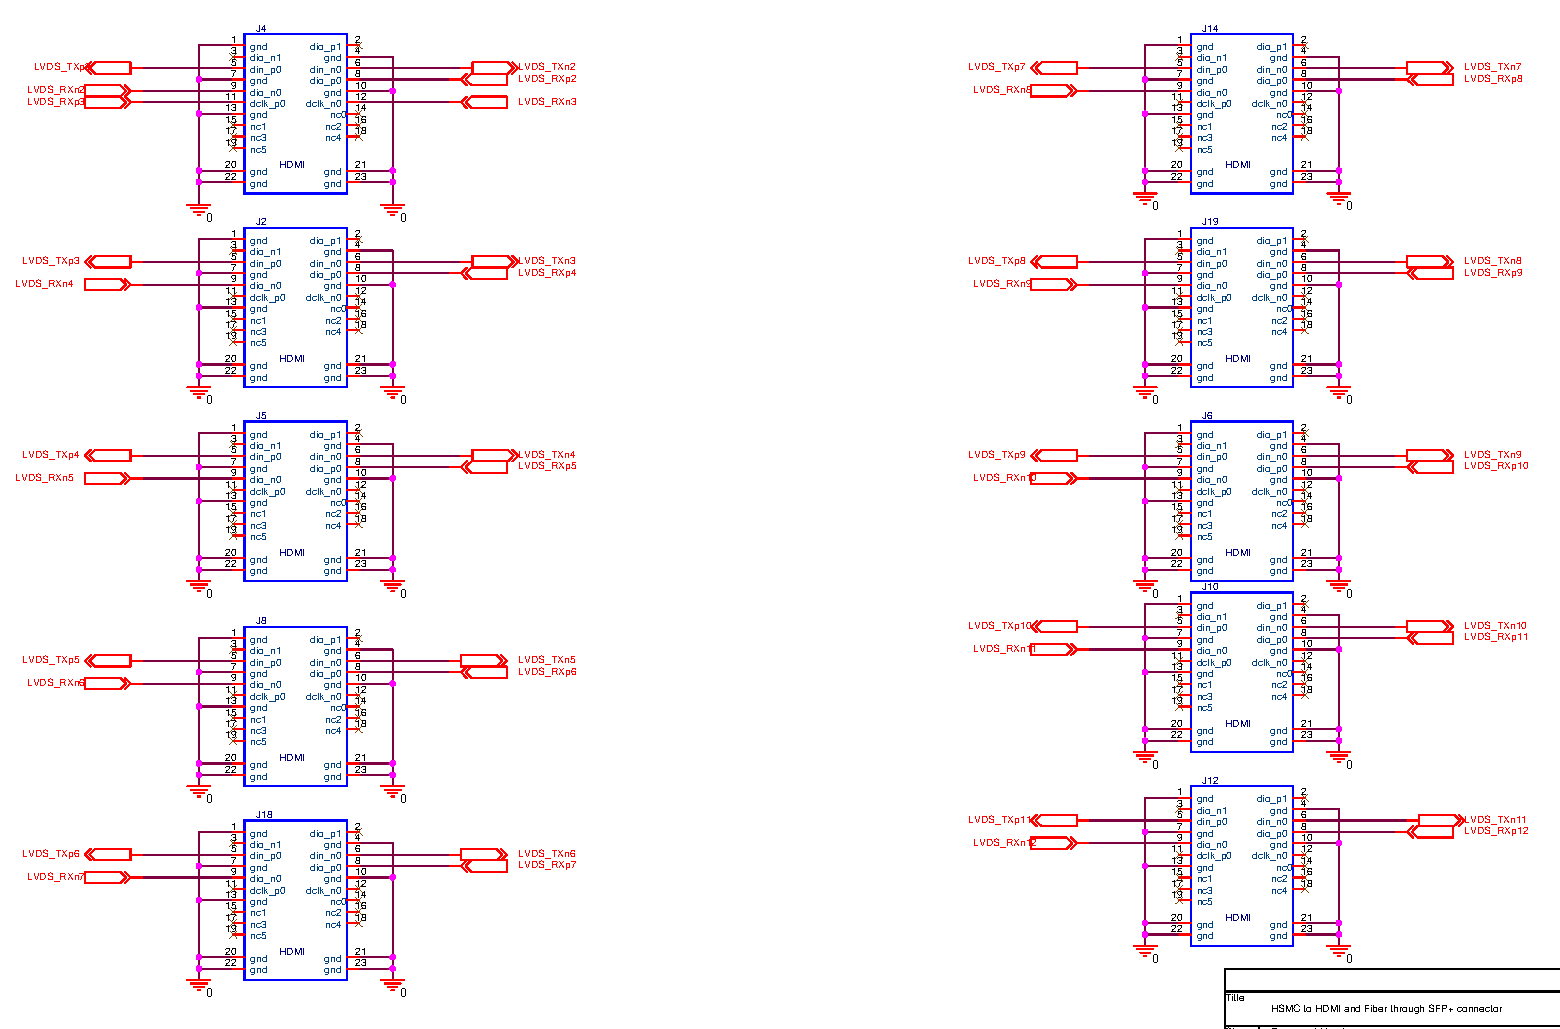
\includegraphics[width=1\linewidth]{../img/pcb_sch2}
\caption{PCB Schematic, HDMI connectors.}
\label{fig:pcb_sch2}
\end{center}
\end{sidewaysfigure}

\begin{sidewaysfigure}[H] % H(strictly put HERE > h!)
\begin{center}
% h(here), !(force), t(top), b(bottom), p(on extra page)
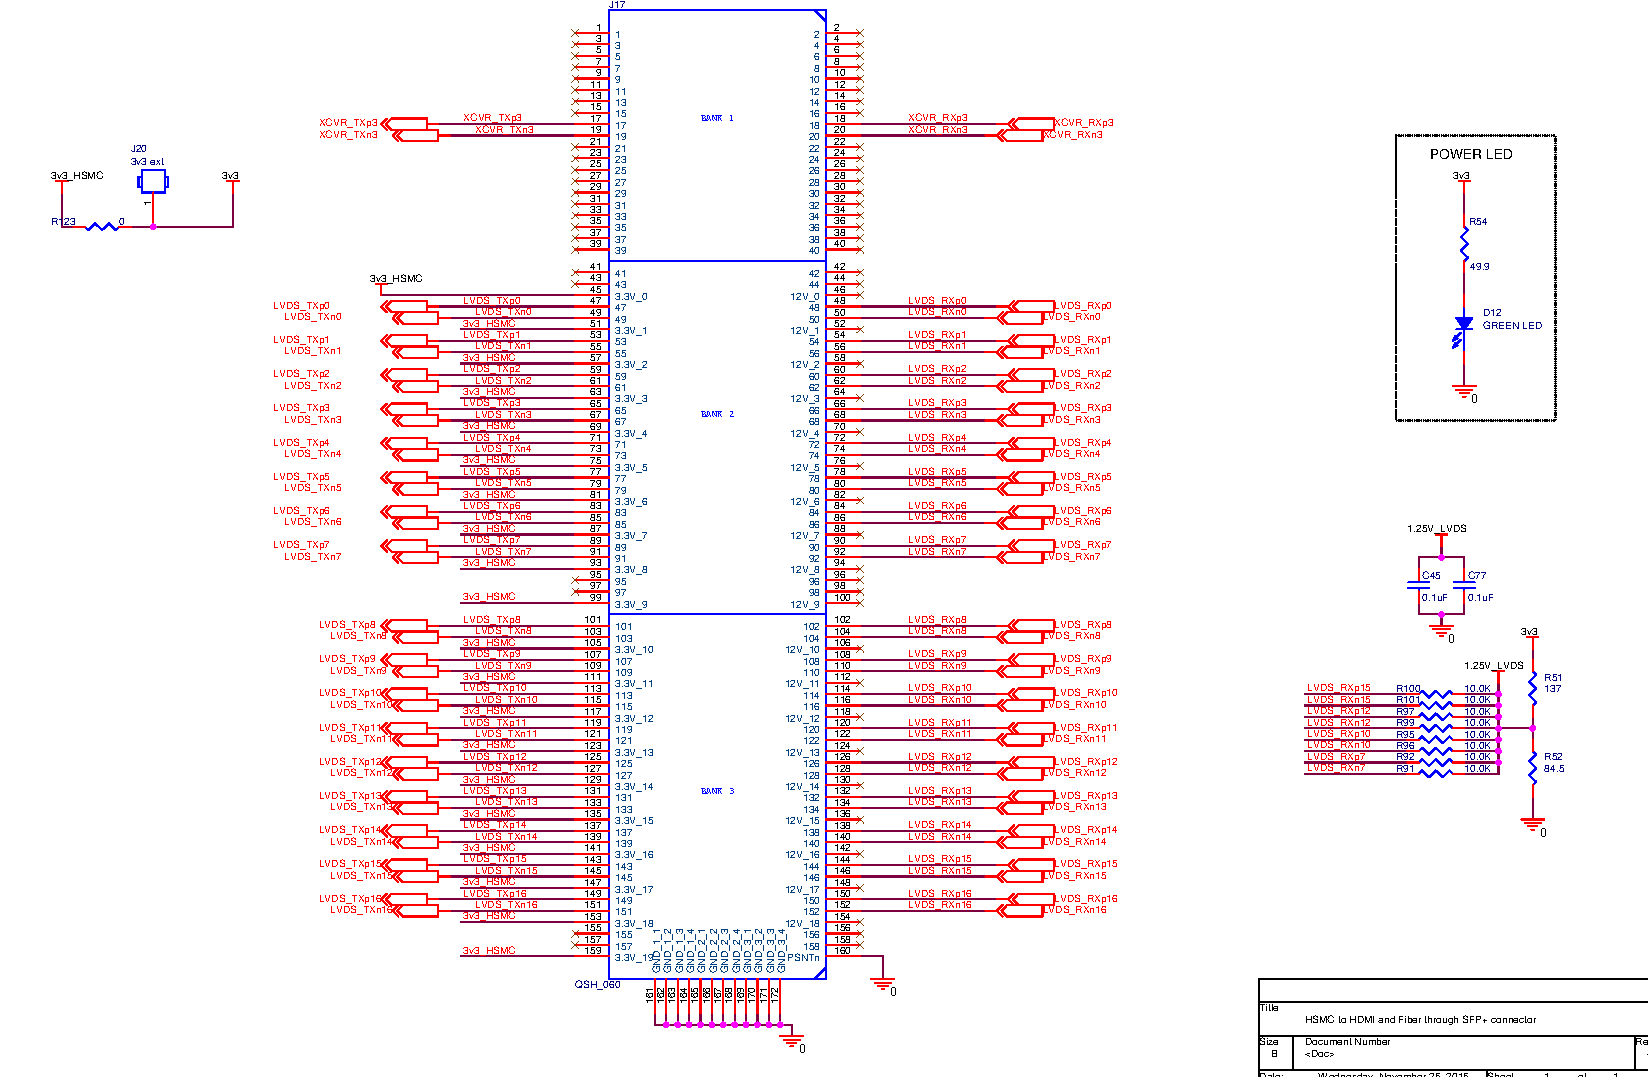
\includegraphics[width=1\linewidth]{../img/pcb_sch3}
\caption{PCB Schematic, HSMC connector.}
\label{fig:pcb_sch3}
\end{center}
\end{sidewaysfigure}

\begin{figure}[]
    \centering
    \begin{subfigure}[t]{0.7\textwidth}
        \centering
        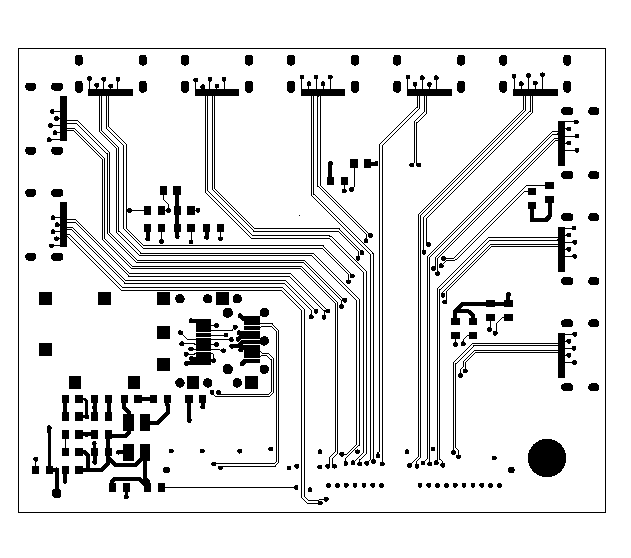
\includegraphics[width=\linewidth, angle=0]{../img/pcb_top}
        \caption{Copper top.}
    \end{subfigure}%
    \\
    \begin{subfigure}[t]{0.7\textwidth}
        \centering
        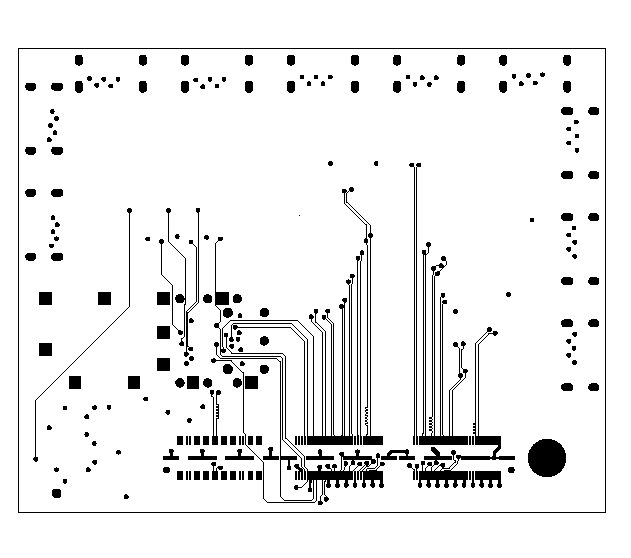
\includegraphics[width=\linewidth, angle=0]{../img/pcb_btm}
        \caption{Copper bottom.}
    \end{subfigure}
    \caption{PCB Layout, top and bottom layers.}
    \label{fig:pcb_tb}
\end{figure}

\begin{figure}[]
    \centering
    \begin{subfigure}[t]{0.7\textwidth}
        \centering
        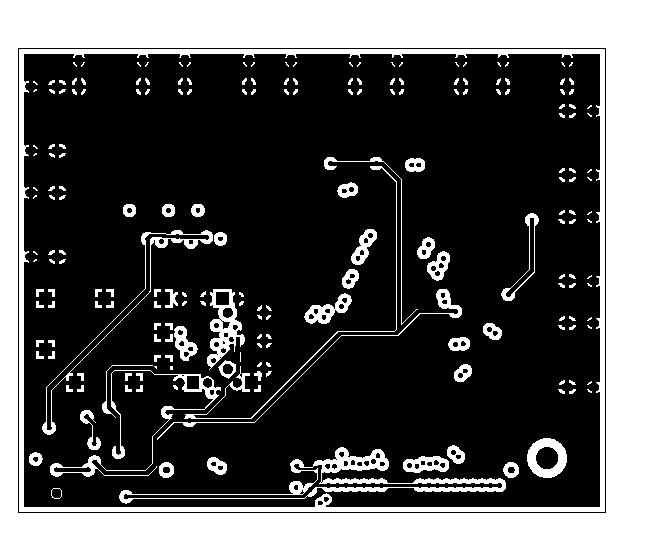
\includegraphics[width=\linewidth, angle=0]{../img/pcb_in1}
        \caption{Inner layer: voltage.}
    \end{subfigure}%
    \\
    \begin{subfigure}[t]{0.7\textwidth}
        \centering
        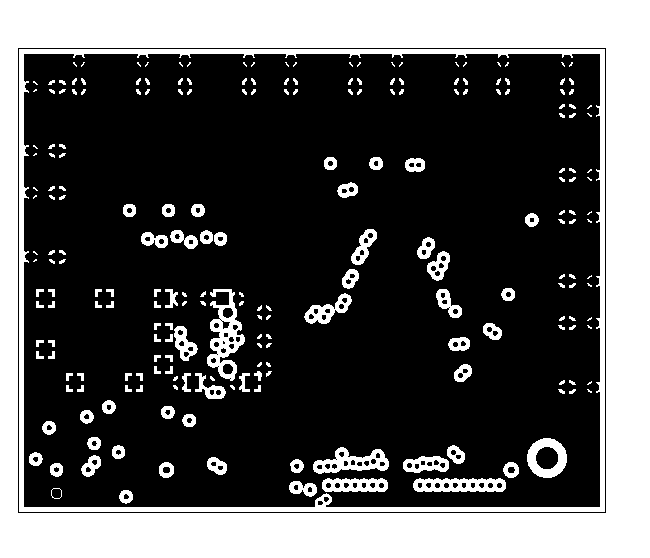
\includegraphics[width=\linewidth, angle=0]{../img/pcb_in2}
        \caption{Inner layer: ground.}
    \end{subfigure}
    \caption{PCB Layout, inner layers.}
    \label{fig:pcb_in}
\end{figure}

\end{document}
